\documentclass{article}
\usepackage[utf8]{inputenc}
\usepackage{titling}
\usepackage{graphicx}
\usepackage{xcolor}
\usepackage[colorlinks=true,linkcolor=darkgray, urlcolor =gray]{hyperref}
\usepackage[spanish]{babel}
\DeclareUnicodeCharacter{301}{~}
\usepackage{url}
\DeclareUnicodeCharacter{202F}{\,}
\usepackage[T1]{fontenc}


\title{Ejercicios Obligatorios}
\author{Cristina Díaz García}
\date{Diciembre 2018}

\renewcommand\maketitlehooka{\null\mbox{}\vfill}
\renewcommand\maketitlehookd{\vfill\null}


\begin{document}

\addcontentsline{toc}{section}{Índice general}

\begin{titlingpage}
\maketitle

\begin{center}

\includegraphics[scale=0.4]{images/comunicaciones.png} 
\end{center}

\end{titlingpage}

\newpage

\tableofcontents

\newpage

\section{II. Desarrollo de servicios estándar}


\subsection{Ejercicio 1}.

1. Protocolo de transferencia de ficheros trivial (TFTP). Implementar un proceso servidor y un proceso cliente que realicen la transferencia de ficheros sobre UDP de acuerdo al protocolo estándar TFTP definido en el RFC 1350. Tener en cuenta los siguientes puntos.

\begin{itemize}
\item Usar otro puerto diferente al estándar 69 de TFTP para el servidor.
\item La transferencia podrá hacerse en cualquiera de los dos sentidos (get o put). La fase de transferencia de datos y su finalización es igual para ambos procesos cliente y servidor,
variando sólo el establecimiento de la comunicación.
\item El fichero que se transfiera debe ser textual ya que se mostrará por pantalla
(opcionalmente pueden almacenarse los datos transferidos en un fichero).
\item El proceso cliente tendrá un pequeño interfaz de usuario para pedir el tipo de la
transferencia y el nombre del fichero a transferir. Emular los comandos del cliente tftp
estándar (como mínimo: connect, get, put y quit).
\item Tanto el cliente como el servidor comprobarán que todos los mensajes que le llegan han
sido enviados por el proceso correcto (comprobando el identificador de transferencia que
será la IP y el puerto), sino contestará con un mensaje de error. El servidor podrá ser
concurrente o iterativo.
\item Ambos procesos implementarán los mecanismos para garantizar que la transferencia se
haga de forma fiable. Para ello se comprobará que los números de secuencia de los
paquetes sean consecutivos y ante la pérdida de un paquete se retransmitirá después de
esperar 1 segundo. Poner un número máximo de reintentos (ej: 3 o 5).
\item Cada proceso tendrá dos modos funcionamiento: el correcto y con pérdida de paquetes. El
modo de funcionamiento con pérdida de paquetes consiste en que durante el inicio y la
transferencia de un fichero se podrán perder paquetes (acks o datos) hasta un 5\%. La
pérdida de paquetes se hará simulada, cada vez que un proceso cliente o servidor tenga
que enviar un mensaje, de forma aleatoria decidirá si lo envía o no. Al finalizar se dará un
resumen estadístico con el numero/porcentaje de paquetes perdidos y retransmitidos.
\item Por simplicidad no se considerará que el primer paquete enviado (READ o WRITE) pueda
perderse.
\item El proceso cliente (y/o el servidor) dará la traza de la transferencia con el formato que se sigue en el ejemplo:

---> RRQ “fichero.dat” “octet” 		<--- ACK 0\\
---> DATA 1 512 bytes 				<--- ACK 1\\
---> DATA 2 10 bytes				<--- ACK 2 (P)\\
---> DATA 2 10 bytes (R)			<--- ACK 2\\
\% P: paquetes perdidos; \% R: paquetes retransmitidos
\end{itemize}

Este protocolo se ha implementado con diez clases:

\begin{center}
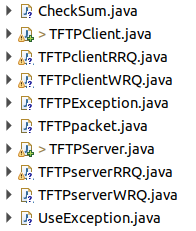
\includegraphics[scale=1]{images/TFTP.png}
\end{center}

\begin{itemize}
\item \textbf{TFTPClient.java:} Es el cliente TFTP como tal. Procesa los argumentos que se le pasan y crea las peticiones, ya sean de escritura (\textit{TFTPclientWRQ}) o de lectura (\textit{TFTPclientRRQ}).
\item \textbf{TFTPException.java:} Excepción genérica de TFTP.
\item \textbf{UseException.java:} Excepción lanzada cuando los argumentos usados no son los correctos.
\item \textbf{TFTPclientRRQ.java:} Abre el documento, lo procesa en bloques de 516 bytes. Hace la función hash del documento haciendo uso de la clase \textit{CheckSum.java} para comprobar que los datos son correctos.
\item \textbf{TFTPclientWRQ.java:} Abre el documento, lo procesa en bloques de 516 bytes y lo escribe en otro archivo. Hace la función hash del documento haciendo uso de la clase \textit{CheckSum.java} para comprobar que los datos son correctos.
\item \textbf{TFTPpacket.java:} Clase que modela un paquete de datos TFTP, con sus distintas variables, sus \textit{getters}, sus \textit{setters} y las funciones que se pueden usar con ellos.
\item \textbf{CheckSum.java:} Función hash con SHA1 del archivo que se le pase como argumento.
\item \textbf{TFTPServer.java:} Es el servidor TFTP como tal. Procesa las peticiones que le llegan, ya sean de escritura (\textit{TFTPserverWRQ}) o de lectura (\textit{TFTPserverRRQ}).
\item \textbf{TFTPserverRRQ.java:} Abre el documento y envía los datos para su lectura. Hace la función hash del documento haciendo uso de la clase \textit{CheckSum.java} para comprobar que los datos son correctos.
\item \textbf{TFTPserverWRQ.java:} Abre el documento y recibe los datos para su escritura. Hace la función hash del documento haciendo uso de la clase \textit{CheckSum.java} para comprobar que los datos son correctos.
\end{itemize}

\section{III. Patrones de diseño}

\subsection{Ejercicio 3}

3. Implementar un servidor multi-cliente de chat, utilizando los canales TCP del paquete NIO
y el Selector. El servidor leerá mensajes de entrada de cada cliente y los difundirá entre todos los canales almacenados en el selector. Dispondrán de una implementación de un cliente de chat con interfaz gráfica que pueden usar para probar la aplicación ó opcionalmente pueden
proporcionar una propia. Se valorará el grado de modularización de la solución presentada.

La solución está implementada con cuatro clases:

\begin{itemize}
\item \textbf{Cliente.java:} Toma como argumento un puerto, y abre una conexión con localhost y ese puerto.
\item \textbf{Server.java:} Se abre la conexión y espera las peticiones de los clientes.
\item \textbf{TCPProtocol.java:} Interfaz que se implementará con \textit{EchoProtocol.java}.
\item \textbf{EchoProtocol.java:} Gestiona el servicio de echo.
\end{itemize}

\end{document}